\documentclass{article}
\usepackage{tikz, comment}
\usepackage{pifont}
\usepackage{fontspec}
\usetikzlibrary{arrows, decorations.markings, decorations.pathreplacing}
\begin{comment}
:Title: Not defined yet
:Tags: approximation by differentials;inverse variation, inverse proportion , inversely proportional ;equation of a line;average rate of change, arc ;area using parametric equations,parametric integral formula
:Prob: 0.4806;0.4091;0.4086;0.4017;0.3859
:Slug: No name yet

Description Here.........
\end{comment}
\begin{document}\centering

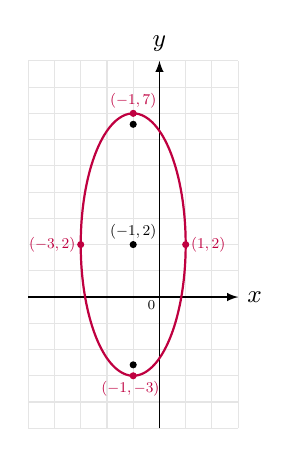
\begin{tikzpicture}[>=latex,xscale=.5/1.5, yscale=.5/1.5][font=\sf\small]

\draw[xstep=1cm,ystep=1cm,color=gray!20] (-5, -5) grid (3, 9);

\draw[->] ({-4-1}, 0) -- ({4-1}, 0)node[right] {\small $x$};
\draw[->] (0, {-7+2}) -- (0, {7+2})node[above] {\small $y$};

\clip[] (-5, -5) rectangle (3, 9);

\draw[purple, thick, samples=100, smooth, domain=0:2*pi, variable=\t]
plot ({-1+sqrt(4)*cos(\t r)}, {2+sqrt(25)*sin(\t r)});

%\node[purple, xshift=-50, yshift=20, scale=0.6] at (0,0) {$y^2+2y+12x+25 = 0$};

\draw[black, fill, xscale=1.5, yscale=1.5] ({-1/1.5}, {2/1.5}) circle(0.075)node[above, xshift=0, yshift=0, scale=0.6] {$(-1,2)$};

\draw[black, fill, xscale=1.5, yscale=1.5] ({-1/1.5}, {(2+sqrt(21))/1.5}) circle(0.075);
\draw[black, fill, xscale=1.5, yscale=1.5] ({-1/1.5}, {(2-sqrt(21))/1.5}) circle(0.075);

\draw[purple, fill, xscale=1.5, yscale=1.5] ({-1/1.5}, {(2+5)/1.5}) circle(0.075)node[above, xshift=0, yshift=0, scale=0.6] {$(-1,7)$};
\draw[purple, fill, xscale=1.5, yscale=1.5] ({-1/1.5}, {(2-5)/1.5}) circle(0.075)node[below, xshift=-1, yshift=0, scale=0.6] {$(-1,-3)$};

\draw[purple, fill, xscale=1.5, yscale=1.5] ({(2-1)/1.5}, {2/1.5}) circle(0.075)node[right, xshift=0, yshift=0, scale=0.6] {$(1,2)$};
\draw[purple, fill, xscale=1.5, yscale=1.5] ({(-2-1)/1.5}, {2/1.5}) circle(0.075)node[left, xshift=0, yshift=0, scale=0.6] {$(-3,2)$};

\node[scale=0.7] at (-0.2*1.5, -0.2*1.5) {\scriptsize$0$};

\end{tikzpicture}
\end{document}